\documentclass{article}%
\usepackage[T1]{fontenc}%
\usepackage[utf8]{inputenc}%
\usepackage{lmodern}%
\usepackage{textcomp}%
\usepackage{lastpage}%
\usepackage[head=40pt,margin=0.5in,bottom=0.6in]{geometry}%
\usepackage{graphicx}%
%
\title{\textbf{“Cifras de Reverol contrastan con la realidad del país”}}%
\author{ZULVYN DÍAZ}%
\date{28/11/2018}%
%
\begin{document}%
\normalsize%
\maketitle%
\textbf{URL: }%
http://www.el{-}nacional.com/noticias/sucesos/cifras{-}reverol{-}contrastan{-}con{-}realidad{-}del{-}pais\_261330\newline%
%
\textbf{Periodico: }%
EN, %
ID: %
261330, %
Seccion: %
Sucesos\newline%
%
\textbf{Palabras Claves: }%
NO\_TIENE\newline%
%
\textbf{Derecho: }%
CONTEXTO%
, Otros Derechos: %
NO\_TIENE%
, Sub Derechos: %
NO\_TIENE%
\newline%
%
\textbf{EP: }%
NO\newline%
\newline%
%
\textbf{\textit{Roberto Briceño{-}León señaló que la criminalidad ha variado a consecuencia de la situación. Los afectados son los ciudadanos de a pie}}%
\newline%
\newline%
%
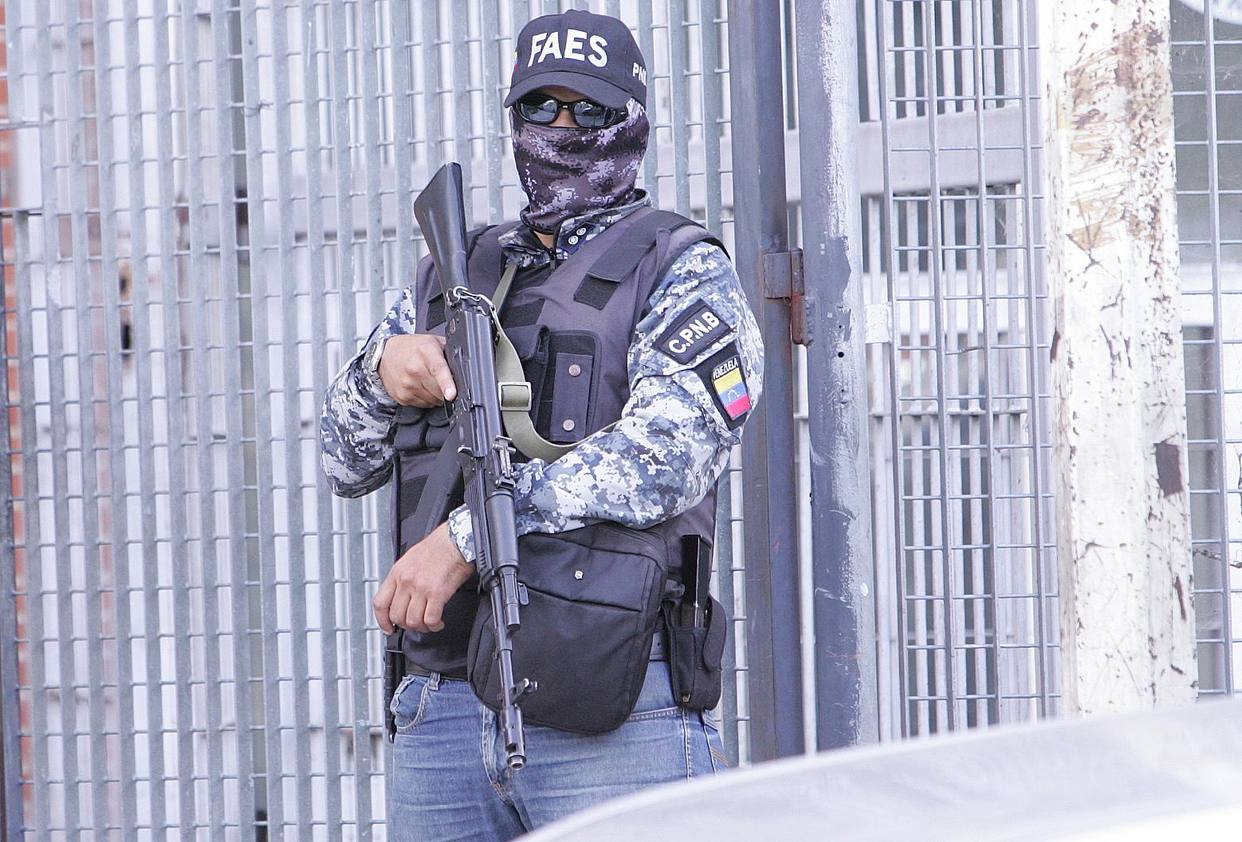
\includegraphics[width=300px]{242.jpg}%
\newline%
%
Néstor Reverol, ministro de Interior, Justicia y Paz, presentó un reporte de seguridad de 2018 según el cual hubo una reducción de 28,4\% de la incidencia delictiva en todo el ámbito nacional, en comparación con el mismo período en 2017.%
\newline%
%
La tasa de homicidios de 30 por cada 100.00 habitantes disminuyó 17 puntos en relación con la del año 2017, cuando fue de 47 por cada 100.000 habitantes lo que equivale a una reducción de la criminalidad de 27,7\%, afirmó el ministro.%
\newline%
%
Para el sociólogo Roberto Briceño{-}León, director del Observatorio Venezolano de la Violencia, las cifras presentadas “difieren de las que hasta ahora ha reportado al Observatorio Venezolano de la Violencia, y distan mucho del sentir y la experiencia diaria de los venezolanos de a pie que no se sienten más seguros caminando por las calles”. Aseguró que hay delitos que han disminuidos debido a la crisis, como el robo de vehículos.%
\newline%
%
Reverol aseguró: “Se han dejado de cometer 3.703 homicidios, 16.320 hurtos en general y 4.440 hurtos de vehículos”. Destacó que en secuestros a escala nacional la reducción fue de 38,3\%, mientras que para el Distrito Capital la disminución de estos delitos fue de 37,4\%.%
\newline%
%
El ministro señaló que~89,5\% de los delitos de secuestros se concentra en los estados~Miranda,~Aragua~y en la ciudad capital, donde los secuestros disminuyeron en 37,4\%; sin embargo, Briceño{-}León considera que en materia de secuestros resulta difícil determinar si hubo reducción, ya que estos son delitos que no se denuncian y varían en las formas de su ejecución.%
\newline%
%
En cuanto a la disminución de la incidencia delictiva, concluyó que “el delito muta” y se ajusta a la realidad del país. Más que una reducción de la incidencia, es un cambio en la ejecución y modalidad, aseguró.%
\newline%
%
\end{document}